\textit{Feather-trace} \cite{brandenburg2007feather} est outil de suivi d'événements léger conçu pour être intégré dans des applications,  systèmes d'exploitation ou systèmes embarqués. Il est dans notre cas, à la fois intégré dans le noyau modifié \litmus, mais aussi dans les algorithmes d'ordonnancement que nous implémenterons. Il a été choisi pour sa simplicité et sa légèreté. Il permet d'enregistrer sous forme de fichier de log de multiples données de l'ordonnancement, par exemple l'arrivée d'une nouvelletâche, le début d'un nouveau job de cettetâche, la date de la fin d'exécution, et bien d'autres événements. De multiples \textit{wrapper} des fonctions de base de \textit{feather-trace} sont fournie dans \litmus afin de pouvoir log des informations supplémentaires, comme le processeur depuis lequel l’exécution du log est effectuée ou encore depuis quelle fonction l'appel est fait.

Cela a été très utile lorsque j'ai développé des nouveaux ordonnanceur sous \litmus afin de corriger des erreurs. Mais cet outil m'a aussi été essentiel afin de comprendre comment fonctionnait les algorithmes d’ordonnancement fournis avec \litmus. J'ai aussi pu comprendre comment le noyau Linux communiquait avec les ordonnanceur en activant des sorties de debug additionnels dans la configuration du noyau.

Enfin, des outils permettant d'extraire, de synthétiser ou de tracer des graphique de certaines données de ces fichiers de logs sont mis à notre disposition sur un dépôt de code présent sur github nommé \textit{feather-trace-tools}. Voici un exemple du tracé de l'ordonnancement réel de C-EDF :


\begin{figure}[H]
     \centering
     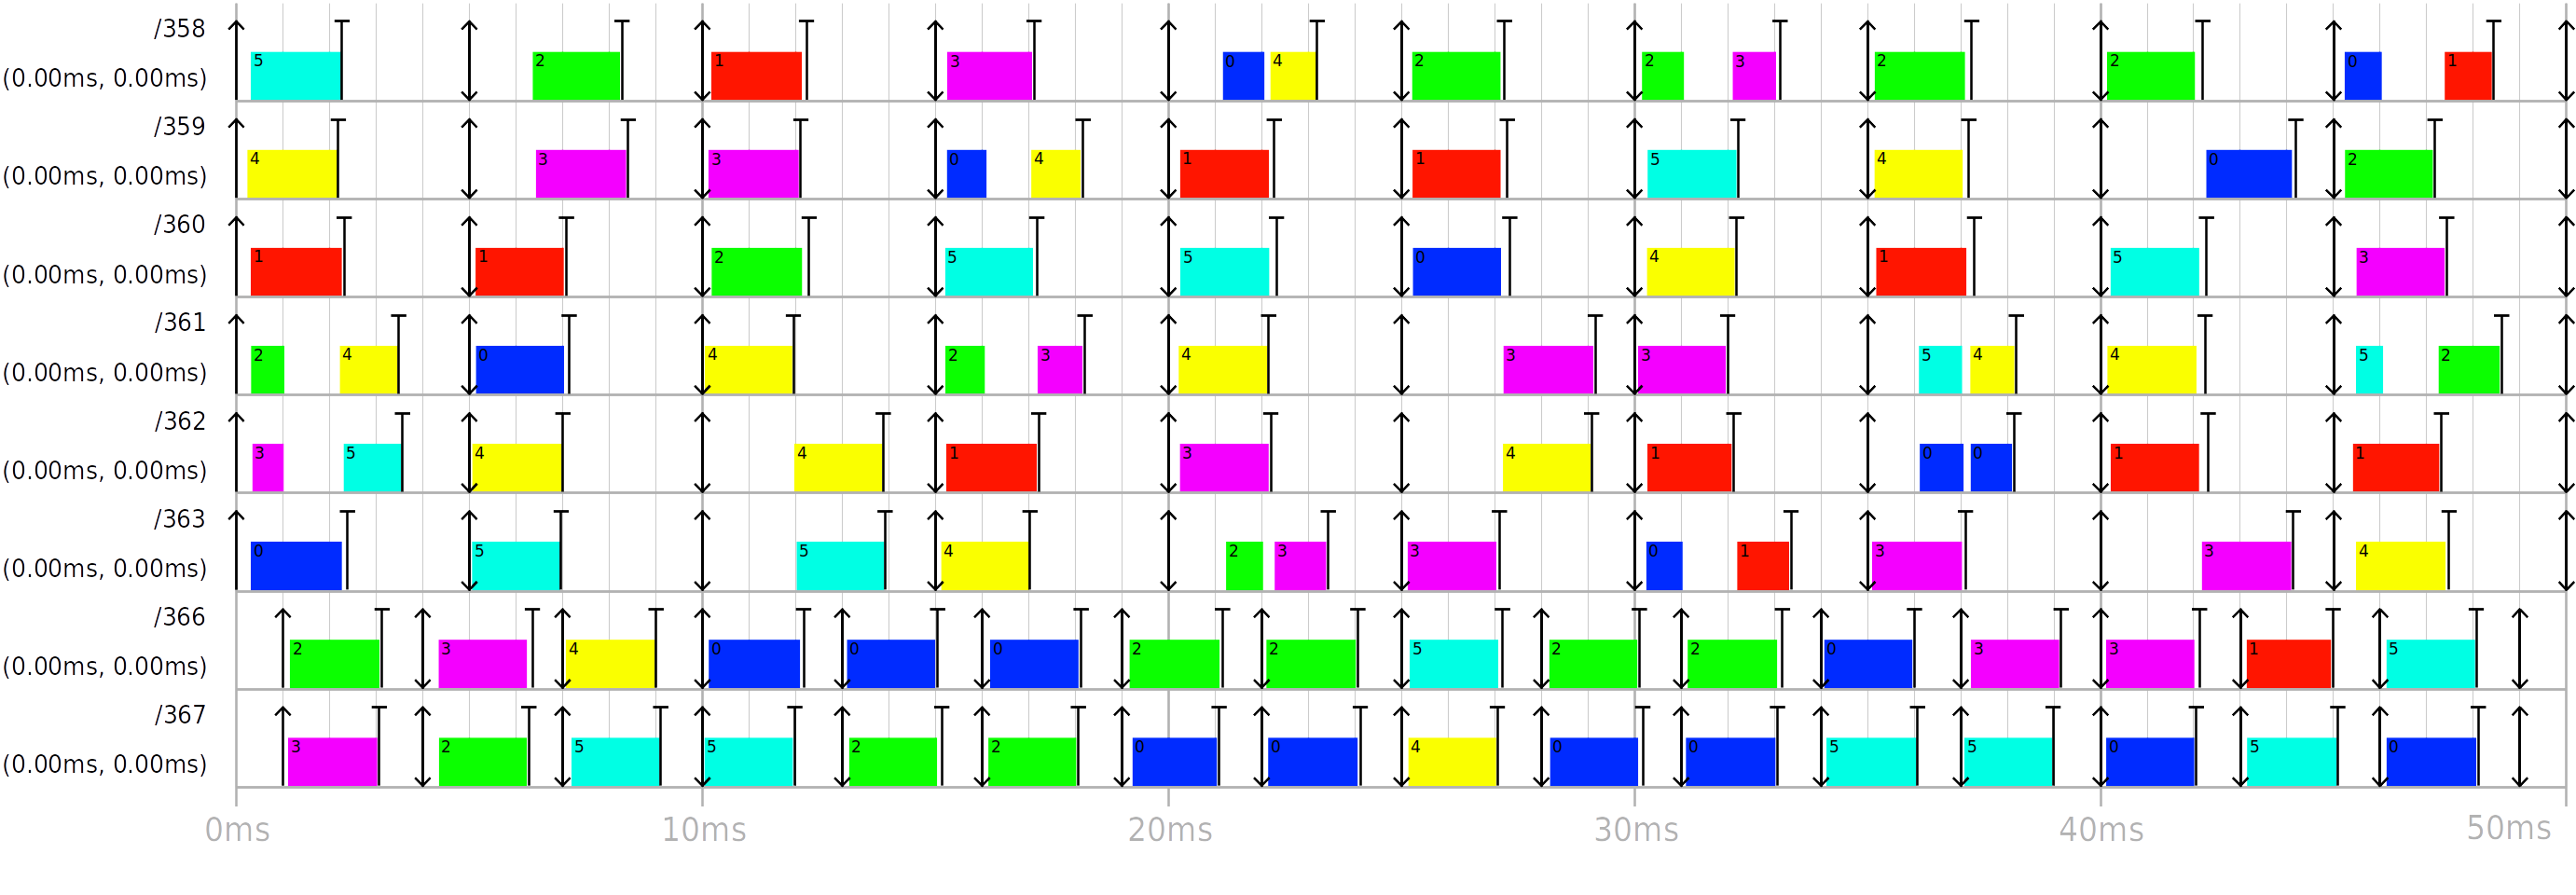
\includegraphics[width=\textwidth]{Images/schedule_host=rock960_scheduler=C-EDF_trace=C-EDF-OFFSET.png}
     \caption{Tracé de l'ordonnancement réel de C-EDF avec 8tâches sur les 6 processeurs}
     \label{fig:trace-cedf}
\end{figure}


Pour cela, les temps d'exécution, les débuts et les fins de chaque jobs s'exécutant sur chaque processeur ont été enregistrés sur la carte de développement avec l'outil \texttt{st-trace-schedule} du dépôt de code mentionnée précédemment. Cet outil générer autant de fichiers que de processeurs sont présents. On peut alors tracer l’exécution réel avec cette fois ci l'outil \texttt{st-draw} en lui fournissant les fichiers générés au préalable. Ici une durée de 50ms a aussi été donnée en argument afin de limiter la durée du tracé.